% Senior Project Notes for Computer Science and Mathematics
% Matthew Lad
% January-March 2022

\documentclass[10pt]{article}

\usepackage{cite}
\usepackage[utf8]{inputenc}
\usepackage[top    = 2.75cm,
			 bottom = 2.50cm,
  			 left   = 3.00cm,
  			 right  = 2.50cm]{geometry}
\usepackage{amsmath}
\usepackage{mathtools}
\usepackage{musixtex}
\usepackage{titling}
\usepackage{graphicx}
\usepackage{marvosym}
\usepackage{multirow}
\usepackage{float}

\graphicspath{{./Images/}}

\setlength\parindent{20pt}

\setlength{\droptitle}{-5em}
 

%---------------------------------INFO----------------------------------------------------------
\title{
    \textbf{Fourier Analysis and Musical Signal Processing}}
\author{\textbf{Matthew Lad}}
\date{Jan.-Mar. 2022}

% Doc. begin
\begin{document}
 
%----------------------------TITLE--------------------------------------------
\maketitle

%------------------------INTRODUCTION--------------------------------------------
\section{Introduction}
\hspace{\parindent} The goal of this paper is to explore the application of Fourier analysis in signal processing and specifically the analysis of music. The mathematical background of music and Fourier analysis will be covered as well as the Fast Fourier Transform (FFT) algorithm and applications of the FFT on musical signals. Along with the mathematics, explorations will be done through computer algorithms.

%----------------------PRELIMINARIES-------------------------------------
\section{Musical and Mathematical Preliminaries}

%-------------------------MUSIC---------------------------------------------------------
\subsection{Musical Preliminaries}
\subsubsection{Sound}
\hspace{\parindent}Although \textbf{sound} is a aural concept, for this paper we will define it as a series of oscillating low and high air pressures. A \textbf{cycle}, or \textbf{vibration}, is one high-pressure and one low-pressure area together. The \textbf{frequency} or \textbf{pitch} is the number of cycles per second, measured in \textbf{Hz} \cite{hertzDefinition}. The higher the frequency of the sound, the higher the pitch of the sound heard. The \textbf{volume}, \textquotedblleft\textbf{loudness}", or \textbf{amplitude} of a sound is defined by the difference in air pressure between a low area and high area of a cycle. A quiet sound can be described as a transition between two densities of similar value. Likewise, a loud sound is a transition between a very high density and a very low density \cite{boatwright1956musictheory} \cite{lenssen2014fouriermusic}. These terms oscillating, cycles, frequencies, etc. are all terms used when dealing with certain functions in mathematics. A diagram of this relation is shown in figure \ref{fig:sound wave 1}. The elementary \textbf{sine} function graphs the air density over time. As the density grows, the sine wave likewise increases.

\begin{figure}[h]
    \centering
    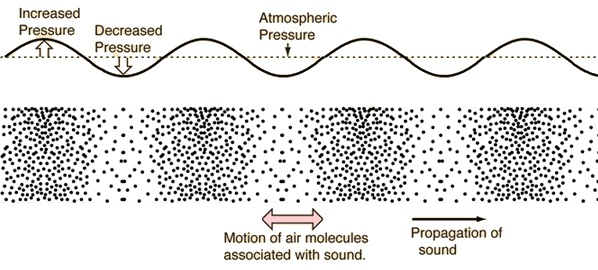
\includegraphics[width=0.7\textwidth]{Sound Waves JPG}
    \caption{The high and low air pressures of sound can be represented by a wave function \cite{nave2017hyperphysics}.} 
    \label{fig:sound wave 1}
\end{figure}

Different notes are determined by specific frequencies. The lower sounding a note is, the lower the frequency the sound wave. Similarly with high-pitched sounds, their frequencies are much higher. The most common system in western music for determining the frequency values of musical notes is a 12-tone system of ratios called \textbf{equal temperament}. Given a reference note with frequency $x$, there are 11 notes between $x$ and $2x$. Each of these notes are separated by a ratio equal to the 12th root of 2, ($\sqrt[12]{2}\approx1.05946$). See figure ?? for a 12-tone scale using equal temperament.

\begin{figure}[h]
	\centering
     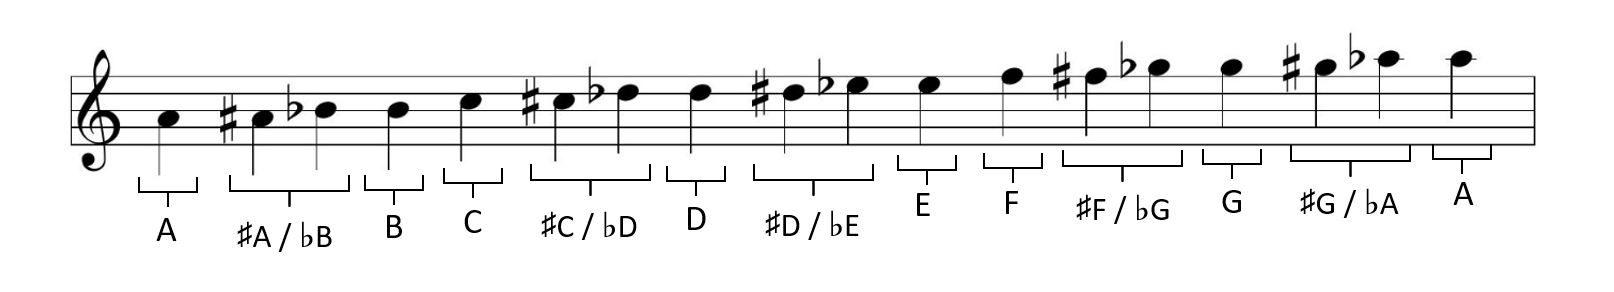
\includegraphics[width=1\textwidth]{MusicalScale}
     \vspace{2mm}
     \begin{tabular}{ |p{2cm}||p{3cm}|p{3cm}|p{3cm}|  }
		\hline
		\multicolumn{4}{|c|}{12-Tone Equal Temperament} \\
 		\hline
 		Note& ISO ALPHA 2 Code &ISO ALPHA 3 Code&ISO numeric Code\\
 		\hline
 		A   & AF    &AFG&   004\\
 		&   AX  & ALA   &248\\
 		B &AL & ALB&  008\\
 		C    &DZ & DZA&  012\\
 		&   AS  & ASM&016\\
 		Andorra& AD  & AND   &020\\
 		Angola& AO  & AGO&024\\
 		\hline
	\end{tabular}
     \caption{The high and low air pressures of sound can be represented by a wave function \cite{nave2017hyperphysics}.} 
     \label{fig:equivalent temperament}
\end{figure}

\vspace{1cm}

The process of determining the frequency value of each note is known as \textbf{tuning}. Western music commonly takes the note $A4=440$Hz as a reference value and then takes ratios from A4 to determine the other frequencies. For example, the note $A4$ has a ratio of $1:1$ with itself, which is $440$Hz. Going to the next whole note, $B5$, the ratio becomes $2:1$ and so $A5=880$Hz.
% show a picture of these two notes on a staff.
The notes $B4, C5, D5, E5, F5, and G5$ lie between $A4$ and $A5$ and are determined by similar ratios. 
% Insert diagram of pitch ratios.
See \cite{tuningSystems},  for more information on tuning.





%%%  Now Explain exactly everything in this video: https://www.youtube.com/watch?v=XPbLYD9KFAo
%%% Ensure the graphs are done correctly, especially ensure the units are accurate. Also understand which time stamp the frequency graph is taken from. https://www.youtube.com/watch?v=RHmTgapLu4s

%%% References^^^^: 
% - Music theory book
% - Two tuning websites (https://www.earmaster.com/music-theory-online/ch06/chapter-6-2.html)
% - frequencies of notes
% - https://en.wikipedia.org/wiki/Equal_temperament
% - 

%%% Ensure that you explore the connections between fourier harmonics and frequencies. See if you can explore this in python with scipy and stuff. You will have to do this after diving into the mathematics.


%-------------------------MATH-----------------------------------------------------------------
\subsection{Mathematical Preliminaries}

%%%% Write a little introduction to the Math stuff.


%-------------------------PERIODIC FUNCTIONS------------------------------------------------------
\subsubsection{Periodic Functions}
\hspace{\parindent} A \textbf{periodic function} is any function for which $f(t) = f(t + T) \: \text{for all} \: t$.
The smallest constant $T$ which satisfies it is called the \textbf{period} of the function (it 'repeats' every $T$) \cite{hsu1970fourier}.

%%%% Talk about your analysis in python and combining notes to try and make a beautiful sound. Emphasize the sine waves.

%%%% Figure out where to go from here.





%-------------------------TIME & FREQUENCY----------------------------------------------------
\subsubsection{Time and Frequency Domains}
\hspace{\parindent} Remembering the sine wave function from figure \ref{fig:sound wave 1}, we will refer to it with $f(t)$. We see that $t$ is time and the value $f(t)$ represents the motion of the low and high-pressure areas. This function $f(t)$ is called the \textbf{time domain representation} because it shows how the sound behaves over time (the x-axis is time and the y-axis is amplitude). Now looking at the graphs in figure \ref{fig:frequency graphs}, we see that the y-axis is also amplitude but the x-axis here is frequency. The functions that create these graphs (which we can arbitrarily call $f(x)$ and $g(x)$) are called \textbf{frequency domain representations} \cite{morrison1994fourier}. As we will see later in this paper, the two domains are closely connected and important through the paper.


% In carrying sound, air acts much like rippling water. When something large like a rock hits the water, a multitude of large and small waves emanate from where it hit the water. Sound, likewise, consists of a multitude of waves in combination. For sounds particular to music, the largest wave present is referred to as the \textbf{fundamental} or \textbf{first partial}. Smaller waves, decreasing in size from the fundamental wave, are know as the \textbf{second, third, fourth, etc. partial}. These partials above the fundamental add to the depth of the sound and make it more enjoyable to listen to. This quality is referred to as the \textbf{timbre} or \textbf{tone quality} of the sound. Instruments and voices vary in tone quality because their various structures emphasize different partials \cite{boatwright1956musictheory} \cite{lenssen2014fouriermusic}.
%
%\begin{figure}[h]
%    \centering
%    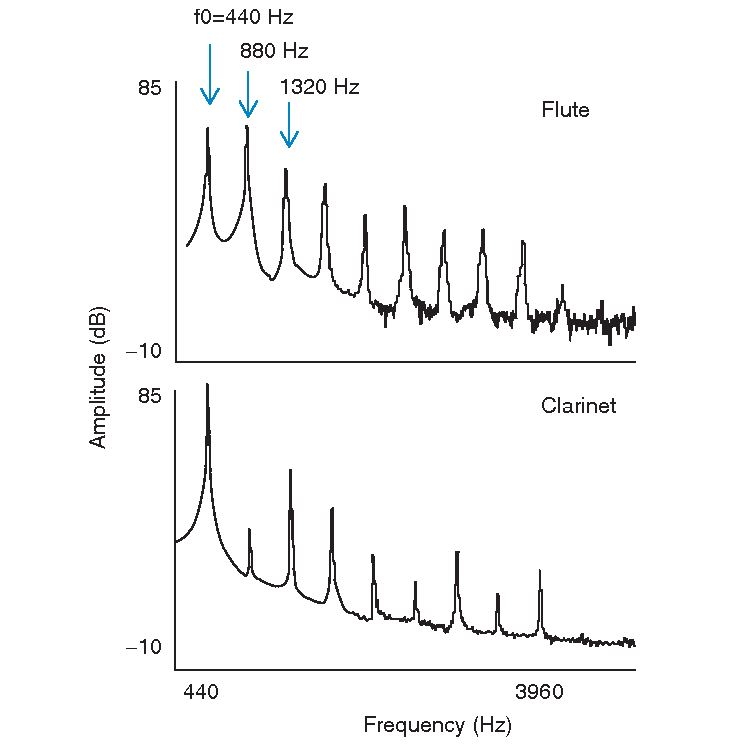
\includegraphics[width=0.7\textwidth]{FluteClarinetFrequencySpectrum}
%    \caption{Graphs of a flute and clarinet playing the same note. The lines represent the amplitude and frequency of sine waves that would create each sound. Each sound is composed of a fundamental (f0) and partials at multiples of the fundamental frequency, highlighted by the arrows in the graph. Note that there are differences in the relative amplitude of different harmonics for flute versus clarinet. This contributes to the timbre, or quality, of the sound and differentiates the sounds of a flute and a clarinet playing the same note. \cite{Lotto2011Psychology}.}
%    \label{fig:frequency graphs}
%\end{figure}



\vspace{7cm}






%-------------------------ORTHOGONALITY------------------------------------------------------
\subsubsection{Orthogonality of Vectors and Functions}
\hspace{\parindent} A \textbf{vector space} is any set that satisfies the defined axioms of addition and scalar multiplication. Details not listed here. An \textbf{inner product} is a function on a vector space which satisfies the following axioms: ($u$ and $v$ and $w$ are vectors in the vector space and $c$ is a scalar) \cite{shields1968linearalgebra}.
\begin{enumerate}
    \item $\langle u, v \rangle = \langle v, u \rangle$
    \item $\langle u, v + w \rangle = \langle u, v \rangle + \langle u, w \rangle$
    \item $c \langle u, v \rangle = \langle cu, v \rangle$
    \item $\langle v, v \rangle \geq 0$, and $\langle v, v \rangle = 0$ if and only if $v = 0.$
\end{enumerate}

\vspace{2mm}

An \textbf{inner product space} is a vector space with a defined inner product which satisfies the above axioms for every vector within it. Properties \& Definitions related to Inner Product Spaces:  \cite{shields1968linearalgebra}.
\begin{enumerate}
    \item $\langle 0, v \rangle = \langle v, 0 \rangle$ = 0
    \item $\langle u + v, w \rangle = \langle u, w \rangle + \langle v, w \rangle$
    \item $c \langle u, v \rangle = \langle u, c v \rangle$
    \item The \textbf{norm} (or \textbf{length}) of $u$ is $||u|| = \sqrt{\langle u, u \rangle}$
    \item The \textbf{distance} between $u$ and $v$ is $d(u, v) = ||u-v||$
    \item The \textbf{angle} between two nonzero vectors $u$ and $v$ is: 
    
    $\cos(\theta) = \frac{\langle u, v \rangle}{\|u\| \|v\|}$, $0 \leq \theta \leq \pi$
    \item Vectors $u$ and $v$ are \textbf{orthogonal} if $\langle u, v \rangle = 0.$
\end{enumerate}

\vspace{2mm}

When a set of vectors $S = \{ u_1, u_2, u_3, ... \}$ satisfies $(u_n, u_m) = 0$ when $n \neq m$, we say that the elements of $S$ are \textbf{mutually orthogonal} and that they form an \textbf{orthogonal basis} for the space spanned by $S$.
Any vector in that space can be represented as a linear combination of those basis vectors  \cite{shields1968linearalgebra}.

\textbf{Sets of functions:} The set of functions $\{f_1(t),\:f_2(t),\:f_3(t),\:...,\:f_k(t),\:...\}$ is orthogonal on an interval $a < t < b$ if for any two functions $f_n(t)$ and $f_m(t)$ in the set, \cite{shields1968linearalgebra}.
\begin{equation} \label{eq:1.18}
    \langle f_n, f_m \rangle = \int_{a}^{b} f_n(t) f_m(t) \,dt = \begin{cases} 0 & \text{for} \:\: n \neq m \\ r_n & \text{for} \:\: n = m \end{cases}
\end{equation}

%--------------------------COMPLEX EXPONENTIALS--------------------------------------
\subsubsection{Complex Exponentials}
Let $z = x + jy$ where $j = \sqrt{-1}$. Some facts from complex algebra used in this paper:  \cite{morrison1994fourier}.
\begin{enumerate}
    \item $z^{\ast} = x - jy\:\:$ (complex conjugate)
    % \item mod($z$) = $|z|$ = $(x^2 + y^2)^{1/2}$ = $(zz^{\ast})^{1/2}$
    % \item arg($z$) = arctan($y/x$)
    % \item $z + z^{\ast}$ = 2 Re($z$) = $2x$
    % \item $z - z^{\ast}$ = $2j$ Im($z$) = $2jy$
    % \item $e^{\pm j \Theta}$ = cos($\Theta$) $\pm$ $j$ sin($\Theta$)
    % \item cos($\Theta$) = [$e^{j\Theta} + e^{-j\Theta}$] / 2
    % \item sin($\Theta$) = [$e^{j\Theta} - e^{-j\Theta}$] / $2j$
\end{enumerate}

\noindent
The complex exponentials $e^{jn\omega_0t}$ together form the set \cite{morrison1994fourier}.
\[ S = \{ ..., e^{-j3\omega_0t}, e^{-j2\omega_0t}, e^{-j\omega_0t}, 1, e^{j\omega_0t}, e^{j2\omega_0t}, ..., e^{jn\omega_0t}, ... \} \]

%-------------------------THM 2.1 ORTHO COMPLEX EXP----------------------------------
\vspace{4mm}
\noindent
\textbf{\underline{Theorem 2.1:} Orthogonality of the Complex Exponentials}

\vspace{2mm}

% There needs to be more explaining/ transition into this vvvvvv

\noindent
The complex exponentials $e^{jn\omega_0t}$ of the above set satisfy the orthogonality condition
\[ \frac{1}{T_0}\int_{-T_0/2}^{T_0/2} e^{jn\omega_0t} e^{jm\omega_0t^{\ast}} \,dt = \begin{cases} 0 & \text{if} \:\: n \neq m \\ 1 & \text{if} \:\: n = m \end{cases}\] where $T_0 = 2\pi / \omega_0$ and $e^{jm\omega_0t^{\ast}}$ is the complex conjugate $e^{-jm\omega_0t}$.

\hspace{1cm}

\noindent
\underline{Proof:}
\begin{equation}   \label{eq:2.19}
\begin{aligned}
    \frac{1}{T_0}\int_{-T_0/2}^{T_0/2} e^{jn\omega_0t} e^{jm\omega_0t^{\ast}} \,dt \: = \:
    \frac{1}{T_0}\int_{-T_0/2}^{T_0/2} e^{jn\omega_0t} e^{-jm\omega_0t} \,dt \: = \:
    \frac{1}{T_0}\int_{-T_0/2}^{T_0/2} e^{jn\omega_0t-jm\omega_0t} \,dt \\
    \: = \: \frac{1}{T_0}\int_{-T_0/2}^{T_0/2} e^{jw_0t(n-m)} \,dt
\end{aligned}
\end{equation}

\noindent
When $n \neq m$, then $n - m$ is a nonzero integer which we shall call $p$, and so \eqref{eq:2.19} continues as
\begin{equation} \label{eq:2.20}
\begin{aligned}
    = \: 
    \frac{1}{T_0}\int_{-T_0/2}^{T_0/2} e^{jp\omega_0t} \,dt \: = \:
    \frac{1}{T_0}\Big[\frac{1}{j\omega_0p} e^{j\omega_0pt}\Big]_{-T_0/2}^{T_0/2} \: = \:
    \frac{1}{T_0}\Big(\frac{e^{j\omega_0p(T_0/2)}}{j\omega_0p} - \frac{e^{j\omega_0p(-T_0/2)}}{j\omega_0p}\Big) \\
    \: = \: \frac{1}{T_0}\Big(\frac{e^{(j\omega_0pT_0)/2}-e^{(-j\omega_0pT_0)/2}}{j\omega_0p}\Big) \: = \: \frac{1}{T_0}\Big(\frac{e^{jp\pi}-e^{-jp\pi}}{j\omega_0p}\Big) \: = \: \frac{e^{jp\pi}-e^{-jp\pi}}{T_0j\omega_0p} \\
    \: = \: \frac{e^{jp\pi}-e^{-jp\pi}}{2\pi j p} \: = \: \frac{(\cos{p\pi}+j\sin{p\pi}) - (\cos{p\pi}-j\sin{p\pi})}{2 \pi j p} \: = \: \frac{\cos{p\pi}+j\sin{p\pi}-\cos{p\pi}+j\sin{p\pi}}{2 \pi j p} \\
    \: = \: \frac{2j\sin{p\pi}}{2\pi j p} \: = \: \frac{\sin{p\pi}}{p\pi} \: = \: 0
\end{aligned}
\end{equation}

\noindent
On the other hand, when $n = m$ then \eqref{eq:2.19} continues as
\begin{equation} \label{eq:2.21}
\begin{aligned}
    \: = \: \frac{1}{T_0}\int_{-T_0/2}^{T_0/2} e^{jw_0t(n-m)} \,dt \: = \: \frac{1}{T_0}\int_{-T_0/2}^{T_0/2} e^{j\omega_0t(0)} \,dt \: = \: \frac{1}{T_0}\int_{-T_0/2}^{T_0/2} e^{0} \,dt  \: = \: 
    \frac{1}{T_0}\int_{-T_0/2}^{T_0/2} \,dt \\
    \: = \: \frac{1}{T_0}[t]\Big|_{-T_0/2}^{T_0/2} \: = \: \frac{1}{T_0}\Big(\frac{T_0}{2} + \frac{T_0}{2}\Big) \: = \: \frac{T_0}{T_0} \: = \: 1
\end{aligned}
\end{equation}

\noindent
And the proof is complete. \quad Q.E.D. \:\:  \cite{morrison1994fourier}.

%---------------------------FOURIER SERIES----------------------------------------------------
\subsubsection{Fourier Series}
\hspace{\parindent} Using this property of orthogonality, let $f_p(t)$ be a periodic function with period $T_0$, and assume it can be expressed as an infinite sum of complex exponentials, that is, that

\begin{equation} \label{eq:2.22}
\begin{aligned}
    f_p(t) \: = \sum_{n=-\infty}^{\infty} F(n) e^{jn\omega_0t}
\end{aligned}
\end{equation}

The complex exponentials on the right-hand side all repeat at least once whenever $t$ is increased by $T_0$, so both sides are periodic with period $T_0$. To obtain the constants $F(n)$, we first multiply both sides by $e^{-jm\omega_0t}$ and integrate

\begin{equation} \label{eq:2.23}
\begin{aligned}
    f_p(t) \: = \sum_{n=-\infty}^{\infty} F(n) e^{jn\omega_0t} \\
    \frac{1}{T_0}\int_{-T_0/2}^{T_0/2} f_p(t) e^{-jm\omega_0t} \,dt \: = \: \frac{1}{T_0}\int_{-T_0/2}^{T_0/2}\sum_{n=-\infty}^{\infty} F(n) e^{jn\omega_0t} e^{-jm\omega_0t} \,dt \\
    \frac{1}{T_0}\int_{-T_0/2}^{T_0/2} f_p(t) e^{-jm\omega_0t} \,dt \: = \: \sum_{n=-\infty}^{\infty} F(n) \Big[ \frac{1}{T_0}\int_{-T_0/2}^{T_0/2} e^{jn\omega_0t} e^{-jm\omega_0t} \,dt \Big] \\
\end{aligned}
\end{equation}

\vspace{3mm}
\noindent
By Theorem 2.1;

\vspace{2mm}
when $n \neq m$ 

\begin{equation} \label{eq:2.24}
\begin{aligned}
    \frac{1}{T_0}\int_{-T_0/2}^{T_0/2} f_p(t) e^{-jm\omega_0t} \,dt \: = \: \sum_{n=-\infty}^{\infty} F(n) \: [0] \: = \: 0
\end{aligned}
\end{equation}

when $n = m$
\begin{equation} \label{eq:2.25}
\begin{aligned}
    \frac{1}{T_0}\int_{-T_0/2}^{T_0/2} f_p(t) e^{-jm\omega_0t} \,dt \: = \: \sum_{n=-\infty}^{\infty} F(n) \: [1] \: = \: F(m)
\end{aligned}
\end{equation}

\noindent
Then replacing $m$ with $n$ we get
\begin{equation} \label{eq:2.26}
\begin{aligned}
    F(n) \: = \: \frac{1}{T_0}\int_{-T_0/2}^{T_0/2} f_p(t) e^{-jn\omega_0t} \,dt
\end{aligned}
\end{equation}

\noindent \cite{morrison1994fourier}

\vspace{4mm}

\noindent
We can summarize all this into 

%---------------------------FOURIER SERIES EQUATIONS-----------------------------------------
\vspace{4mm}
\noindent
\textbf{\underline{Theorem 2.2:} Complex Fourier Series for Periodic Functions}

\vspace{1mm}
Let $f_p(t)$ be periodic with period $T_0$, defined analytically. Then it can also be represented by the infinite series of complex exponentials
\begin{equation} \label{eq:2.27}
\begin{aligned}
    f_p(t) \: = \sum_{n=-\infty}^{\infty} F(n) e^{jn\omega_0t}
\end{aligned}
\end{equation}

where the coefficients $F(n)$ can be found from the analytical definition of $f_p(t)$ as follows:
\begin{equation} \label{eq:2.28}
\begin{aligned}
    F(n) \: = \: \frac{1}{T_0}\int_{-T_0/2}^{T_0/2} f_p(t) e^{-jn\omega_0t} \,dt \:\:\:\:\:\: (\forall n)
\end{aligned}
\end{equation}

The beginning of section 2.2 to now constitutes the basis for what will be covered in the rest of the paper. To summarize parts of theorem 2.2
\begin{itemize}
    \item Equation \eqref{eq:2.27} is called the \textbf{synthesis equation}.
    \item Equation \eqref{eq:2.28} is called the \textbf{analysis equation}.
    \item The constants $F(n)$ are called the \textbf{complex Fourier coefficients} \cite{morrison1994fourier}.
\end{itemize}

%-------------------------------DISCRETE FOURIER SERIES---------------------------------------
\subsubsection{Fourier Transform}

\hspace{\parindent} Until now, we have looked exclusively at periodic functions of which we can create a Fourier series representation. The question arises if single pulse functions which do not repeat over a period can be represented by Fourier series as well. The side of Fourier analysis dealing with single pulses primarily deals with the \textbf{Fourier transform}.

Given a single pulse, we can think of it as being embedded in a single period of a periodic function. We can then have the period $T_0$ tend towards infinity. Even though we have a periodic function, because the period tends toward infinity we essentially eliminate all other pulses but our original single pulse \cite{morrison1994fourier}. There is a great deal of complexity beyond this, but for the purposes of this paper, we will move straight into theorem 3.1.

%-----------------------THEOREM FOURIER TRANSFORM SINGLE PULSE----------------------------
\vspace{3mm}
\noindent
\textbf{\underline{Theorem 3.1:} Fourier Transform for a Single Pulse}

\vspace{1mm}
\noindent
\hspace{2mm}(provided that the integrals exist:)

\textbf{Synthesis:}
\begin{equation} \label{eq:3.15}
\begin{aligned}
    f(t) \: = \: \frac{1}{2\pi}\int_{-\infty}^{\infty} F(\omega) e^{j\omega t} \,d\omega
\end{aligned}
\end{equation}

\textbf{Analysis:}
\begin{equation} \label{eq:3.16}
\begin{aligned}
    F(\omega) \: = \: \int_{-\infty}^{\infty} f(t) e^{-j\omega t} \,d\omega
\end{aligned}
\end{equation}

\vspace{2mm}
Equation \eqref{eq:3.16} shows that a time domain function $f(t)$ can be \textbf{analyzed} to give an associated frequency domain function $F(\omega)$ that contains all the information in $f(t)$. $F(\omega)$ is known as the \textbf{Fourier transform} of $f(t)$. Likewise, in equation \eqref{eq:3.15} we can see that we can \textbf{synthesize} a pulse given it's Fourier transform function. $f(t)$ then is called the \textbf{inverse Fourier transform} of $F(\omega)$ \cite{morrison1994fourier}.

An amazing feature of the Fourier transform/ inverse Fourier transform is they can be used to operate on all pulse cases. One-time pulses of finite duration, one-time pulses of infinite duration, and periodic functions that inherently have infinite duration can all be analyzed/ synthesized.


% Diagram on page 67 of the text book where it has the two squares for time and frequency domains. You need to put that in here cause its amazing.

% Maybe put an example of an actual problem being solved. Like ex.3.1 on page 70.

%---------------------------SAMPLING------------------------------------------------------
\subsection{Sampling}
\hspace{\parindent} In order to store music and sound on computers, the entire signal must be broken down into a digital format. This consists of sampling the signal at a regular interval, essentially converting the continuous signal into a discrete signal. Saying $s(t)$ is a signal input function, the sampled version of it is a list of $s(t)$ values taken every $T$ seconds. $s(nT)$ is the sampled function, where$T$ is the \textbf{sampling period} and $n$ is an integer. The average number of samples taken in one second is the \textbf{sampling frequency} $f_s=1/T$.

% References for ^^^:
% https://books.google.com/books?id=jxXDQgAACAAJ&q=Communications+Standard+Dictionary
% https://books.google.com/books?id=4z3BrI717sMC

%-----------------------------DISCRETE FOURIER TRANSFORM----------------------------------
\subsection{Discrete Fourier Transform}
\hspace{\parindent} Combining the concepts of the continuous Fourier Transform in section 4.1 with sampling, there is a Fourier Transform that works on sampled functions. Before jumping in, there is some background math that needs to be covered. 

Theorem?:

\textbf{Analysis:}
\begin{equation} \label{eq:3.4.1}
\begin{aligned}
    F_k \: = \: \sum_{n=-\frac{N}{2}+1}^{N/2} \: f_n e^{-j2\pi nk/ N}
\end{aligned}
\end{equation}

\textbf{Synthesis:}
\begin{equation} \label{eq:3.5.1}
\begin{aligned}
    f_k \: = \: \sum_{n=-\frac{N}{2}+1}^{N/2} \: F_n e^{j2\pi nk/ N}
\end{aligned}
\end{equation}

%---------------------------DIRAC DELTA FUNC-----------------------------------------------
\subsection{Dirac Delta Function}

\[ \delta(t) = \begin{cases} \infty & \text{if} \:\: t = 0 \\ 0 & \text{if} \:\: t \neq 0 \end{cases}\]

\vspace{7cm}







%------------------------METHODOLOGY, ALGORITHM, ETC.------------------------------
\section{Methodology, Algorithm, Etc.}

%-----------------------TIME & FREQUENCY DOMAINS---------------------------------------
\subsection{Time and Frequency Domain Analysis}

%----------------------------TIME FROM SINE WAVE--------------------------------------
\subsubsection{Time Domain of a Periodic Signal}

\noindent(more to be added)

%----------------------------FREQUENCY FROM SINE WAVE--------------------------------------
\subsubsection{Time Domain of a Periodic Signal}

\noindent(more to be added)


% You should show an xyz graph to show the relation between time and frequency. it would be pretty cool to show the graph of that as a colorful surface.


%---------------------------TIME IN REAL TIME-------------------------------------------
\subsubsection{Time Domain of a Real Time Signal}
\hspace{\parindent} In order to visualize music, the audio signal must be broken down so that various aspects of the sound can be analyzed. The most sensible first steps would be to look at the musical signal in the time and frequency domains. The time domain can be easily obtained without much math with the help of a python library. Using the library PyAudio, the microphone can be accessed and sound input can be read and manipulated. The library takes in the microphone data as samples and graphs the samples in real time. The x and y axes are time and amplitude. Figure \ref{fig:time_1} shows work done so far in real-time sound analysis. The code starts off by opening a PyAudio "stream." This object takes in microphone data and organizes it into chunks. The chunks are loaded into a buffer and the graphing library, matplotlib.pyplot, then takes the buffer and graphs it. There is also some data manipulation to get the microphone raw data into a graph-able format but details are unimportant for the scope of this paper. The Python, PyAudio, and PyPlot versions used here and throughout the rest of the paper are 3.7.7, 0.2.11, and 3.5.1 respectively \cite{hunter2007pyplot} \cite{pyaudio} \cite{python}. Figure \ref{fig:time_2} shows another such graph.

\begin{figure}[H]
    \centering
    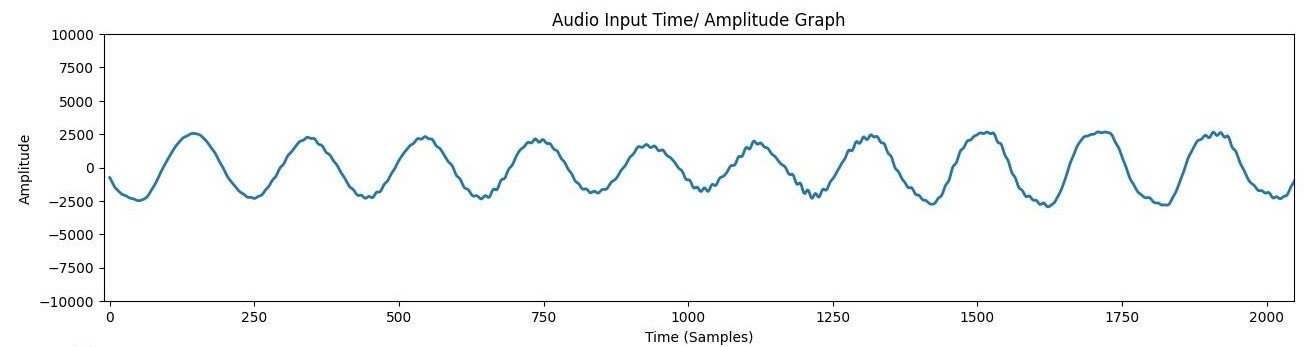
\includegraphics[width=1.05\textwidth]{Alan_1}
    \caption{A graph of the amplitude over time of the author singing a note somewhere between G4 and A4 \cite{noteFrequencies}}
    \label{fig:time_1}
\end{figure}

\begin{figure}[H]
    \centering
    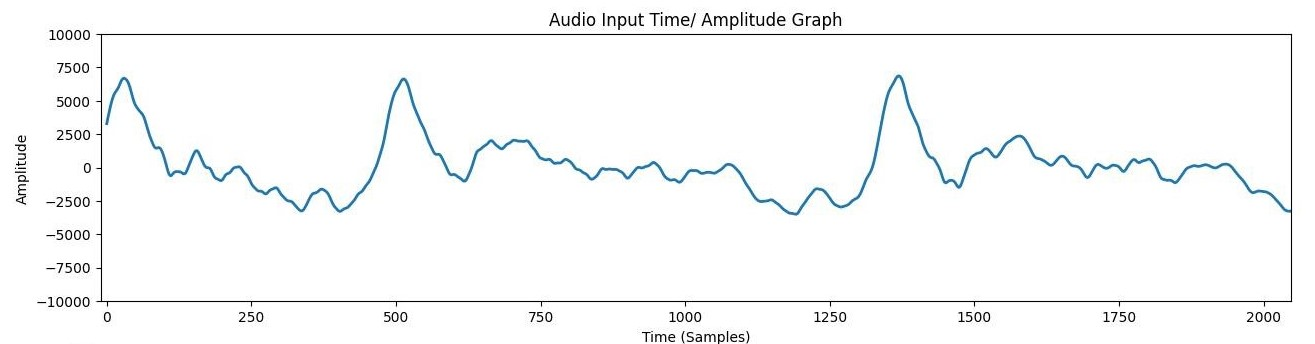
\includegraphics[width=1.05\textwidth]{Matt_1}
    \caption{A graph of the amplitude over time of the author and the author's friend trying to harmonize.}
    \label{fig:time_2}
\end{figure}

%---------------------------FREQUENCY IN REAL TIME-------------------------------------
\subsubsection{Frequency Domain of a Real Time Signal}
\noindent\hspace{\parindent}The next step in this direction is to look at the frequency domain. Taking the same exact signals as shown in figures \ref{fig:time_1} and \ref{fig:time_2} a library called SciPy can be used to go from the time domain to the frequency domain. With the fast Fourier trasform (FFT) build into SciPy, the frequencies that make up the signals of figures \ref{fig:time_1} and \ref{fig:time_2} can be extracted. This was a bit more complicated than the previous analysis but luckily all of the mathematical intricacies are handled by SciPy.  \cite{scipy}. 
% YOU NEED TO DESCRIBE EXACTLY HOW SCIPY DOES IT (ONLY WITH REGARDS TO THE PRELIMINARIES DESCRIBED ABOVE)------------------------------------------------------------------------------------------------------------------------------------------------------------------------------------------------------------------------------------------------------------------------------------------------------------------------------------------------------------------------------------------------------------------------------
Figures \ref{fig:frequency_1} and \ref{fig:frequency_2} show the same note and harmony done by the author but instead of plotting the time on the x-axis, the frequency is plotted instead. This is how the author approximated what note was being sung.

\begin{figure}[H]
    \centering
    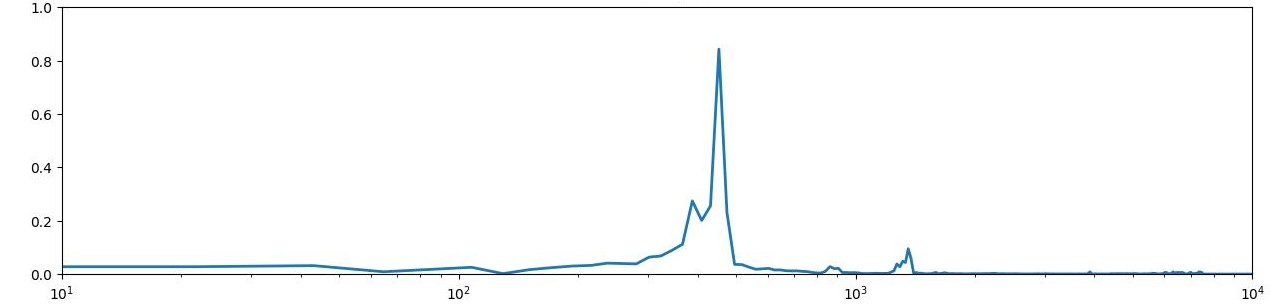
\includegraphics[width=1.05\textwidth]{Alan_1_freq}
    \caption{A graph of the frequencies sung by the author in figure \ref{fig:time_1}}
    \label{fig:frequency_1}
\end{figure}

\begin{figure}[H]
    \centering
    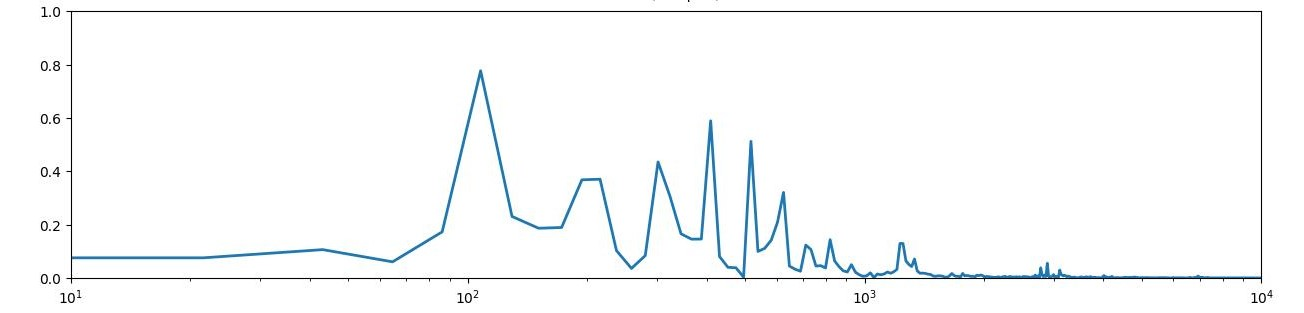
\includegraphics[width=1.05\textwidth]{Matt_1_freq}
    \caption{A graph of the frequencies sung by the author and author's friend's attempted harmony in figure \ref{fig:time_2}}
    \label{fig:frequency_2}
\end{figure}

\noindent(more to be added)

%---------------------EXPECTED OUTCOME-------------------------------------------
\section{Expected Outcome}
\noindent\hspace{\parindent}The expected outcome of this project is to develop a computer program which can take in microphone input, analyze it using Fourier analysis, and then display some form of colorful shapes which represent the musical input. I do not expect the program to be complete by the end of the semester and my main focus of developing this project is in understanding the mathematics behind Fourier analysis and how that math is used in programming, specifically python.

%-----------------------CONCLUSION----------------------------------------------
\section{Conclusion}
\noindent(more to be added)

%-----------------------ACKNOWLEDGEMENTS-----------------------------------------
\section{Acknowledgements}
A Special Thank You To:

\vspace{2mm}\noindent\hspace{\parindent}Dr. Kwadwo Antwi-Fordjour and Dr. Brian Toone for being my project advisors.

\vspace{2mm}\noindent\hspace{\parindent}Samford University for my education.

\vspace{2mm}\noindent\hspace{\parindent}My Family for supporting my education.

\vspace{2mm}\noindent\hspace{\parindent}Alan Crisologo for being the \textquotedblleft author's friend." (See Figure 4)

\vspace{2mm}\noindent\hspace{\parindent}\Cross\hspace{1mm}JMJ\hspace{1mm}\Cross\hspace{2mm}(Jesus, Mary, Joseph)

%------------------------REFERENCES-----------------------------------------------
\bibliography{References}
\bibliographystyle{is-unsrt}


\end{document}
